\chapter{Introducción}
\pagenumbering{arabic}
\setcounter{page}{1}
%\renewcommand{\baselinestretch}{2} %doble espacio paratodo el texto
%\renewcommand{\baselinestretch }{1.5}
 
En esta investigación se realizará la predicción de la respuesta correcta de una pregunta de opción múltiple, este tipo de pregunta de una evaluación requiere de conocimiento previo para ser respondida, mediante técnicas de aprendizaje no supervisado asociado con la experiencia previa. Como experiencia previa se usará las calificaciones anteriores obtenidas de los 2 últimos exámenes de los estudiantes.
\vskip 0.3cm
Para ello se plantea desarrollar un algoritmo de aprendizaje automático no supervisado llamado K-means, el cual sirve para crear clusters. Estos clusters se formarán con la data de las calificaciones  anteriores  de  los  estudiantes. Así  se  obtendría  un  valor  promedio,  Además,  se utilizará técnicas de estadísticas para crear un histograma de las opciones de las preguntas respondidas. Combinando estas 2 técnicas se obtendría un predicción por cada pregunta.
\vskip 0.3cm  
Este proyecto fue pensado debido a la problemática que se tiene al aplicar una evaluación y tener que esperar demasiado tiempo para obtener las respuestas correctas. Pero con lo que se desarrollara se obtendrá la respuesta correcta en corto tiempo.
\vskip 0.3cm 
Para cumplir los objetivos de este proyecto se tendrá primero que investigar acerca del aprendizaje automático no supervisado, así como las técnicas de estadísticas. Luego se desarrollará el algoritmo de aprendizaje automático no supervisado; ya hecho esto se procederá al desarrollo del prototipo de software web para poder ingresar los datos y hacer las pruebas. Finalmente se documentarán los resultados obtenidos.

\section{Justificación de la investigación}
La mayoría de las investigaciones se efectúan con un propósito definido. Tal propósito debe ser lo suficientemente fuerte para que justifique su realización. \cite{Erica}  

\begin{enumerate}
\item[(a)] Razones o motivos e importancia del tema a ser investigado. 
\item[(b)]Sustentar la pertinencia de la pregunta o problema que se abordará en la investigación.
\item[(c)]Considerar los resultados esperados e impactos previstos.
\end{enumerate}



{\bf Ejemplo:}\par

De esta forma, los sistemas integrados para el manejo, tratamiento y disposición final de los RSU que ya existen en diversas ciudades y capitales de los países desarrollados, se hacen referencias para la investigación y justifican posibles adaptaciones para la realidad peruana con el objetivo de que las ciudades sean ambientes más sustentables y competitivos.
\vskip 0.3cm
 Por lo tanto, se puede concluir que realmente existe una necesidad para planificar y modelar una red logística reversa que atienda a las necesidades de una región urbana y que contribuya con la adecuada disposición de los residuos urbanos. A partir del modelamiento es posible estructurar el sistema organizacional, gerencial, operacional y de información de toda la red  de logística reversa, y todas las otras acciones.


\section{Formulación del problema}

  En este trabajo, se propone responder a la siguiente pregunta:
 \begin{center} 
     ¿ Cómo predecir la respuesta correcta de una pregunta de opción múltiple?
 \end{center}


\section{Hipótesis}
Preferentemente para investigaciones explicativas debe ser una respuesta a priori y tentativa guardando coherencia con el problema científico, se formula como una proposición afirmativa, con un lenguaje claro y específico.  Las hipótesis se obtienen por deducción lógica y está sustentada en los conocimientos científicos. \par  
\vskip 0.3cm
{\bf Criterios para formular hipótesis:} \cite{Erica}
\begin{enumerate}
\item[a)] Toda hipótesis de investigación debe ser verificable estadísticamente.  Puede ser difícil o imposible de verificar porque no existe un conocimiento sobre el cual se pueda formular una hipótesis, o bien, porque una o más variables no son medibles.
\vskip 0.2cm
\item[b)] Toda hipótesis debe indicar la relación entre variables, lo que implica que las variables deben ser medibles.
\vskip 0.2cm
\item[c)] Toda hipótesis debe tener sus límites. Pueden escogerse hipótesis que sean sencillas de validar, y sin embargo, altamente significativas.
\vskip 0.2cm
\item[d)] El investigador debe tener una razón específica para considerar una hipótesis, ya sea teórica o por alguna evidencia concreta.    
\end{enumerate}





\section{Objetivos}
Es necesario establecer qué pretende la investigación, es decir, cuáles son sus objetivos. Hay investigaciones que buscan contribuir a resolver un problema en especial, y otras tienen como objetivo principal probar una teoría o aportar evidencia empírica en favor de ella. \par 
\vskip 0.3cm
Segun \cite{Rojas}, los objetivos tienen que expresarse con claridad para evitar posibles desviaciones en el proceso de investigación y deben ser susceptibles de alcanzarse; son las guías del estudio y hay que tenerlos presentes durante todo su desarrollo. Los objetivos deben ser congruentes entre sí.
\vskip 0.3cm
Describir el objetivo central o propósito del proyecto de investigación (debe estar alineado con el problema e hipótesis), así como los objetivos específicos, los cuales deben reflejar los cambios que se esperan lograr en trabajo de tesis (variables). Para estos objetivos específicos utilice verbos como: describir, indicar, modificar, controlar, producir (tecnologías), recuperar, etc..

\subsection{Generales}
\begin{enumerate}
\item[a)] Desarrollar un algoritmo de aprendizaje no supervisado para predecir la respuesta correcta de una pregunta de opción múltiple.
\end{enumerate}


\subsection{Específicos}
\begin{enumerate}
\item[a)] Codificar el algoritmo de aprendizaje no supervisado para trabajar con clusters.
\item[b)] Desarrollar del prototipo de software y aplicarla a la predicción de la respuesta correcta.
\item[c)] Realizar las pruebas y documentar resultados.
\end{enumerate}
\vskip 0.3cm


\section{Estructura de la tesis}

{\bf Ejemplo:}\par
\vskip 0.1cm
El presente trabajo está dividido en cinco capítulos. El primer capítulo presenta los aspectos generales del tema tratado: la formulación del problema, importancia de la investigación, los objetivos, además de la metodología de la investigación y la estructura de la tesis. En el segundo capítulo se contempla los conceptos de predicción, pregunta de opción múltiple y de prototipo de software.

El tercer capítulo trata del tema central de la tesis, diseñándose el algoritmo K-means, se muestra el proceso para hacer la predicción y como se desarrolló el prototipo de aplicación web.

En el cuarto capítulo se presentan los resultados obtenidos en la investigación. En el quinto capitulo se presentan las conclusiones, seguidas de las recomendaciones para futuras investigaciones relacionadas al tema en cuestión. 

Finalmente las referencias bibliográficas usadas para la investigación. Además de los apéndices donde se presentan el algoritmo elaborado, los datos de los resultados y los instrumentos usados para recoger información.

\chapter{Materiales y métodos}

En este capítulo se explica cual fue la metodología empleada para la solución del problema formulado, además de una reseña del material bibliográfico investigado con relación a los temas considerados en esta investigación. Los conocimientos investigados son muy amplios, principalmente aquel que ayudó a consolidar las bases del conocimiento científico para elaborar esta tesis, como lo son los temas de *******************************************
%\vskip 1cm 


\section{Marco teórico}
\subsection{Aprendizaje no supervisado}

\subsubsection{Definición}

Aprendizaje no supervisado es un método de aprendizaje automático donde un modelo es ajustado  a  las  observaciones.  Se  distingue  del  aprendizaje  supervisado  por  el  hecho  de  que no hay un conocimiento a priori. En el aprendizaje no supervisado, un conjunto de datos de objetos de entrada es tratado. Así, el aprendizaje no supervisado típicamente trata los objetos de entrada como un conjunto de variables aleatorias, siendo construido un modelo de densidad para el conjunto de datos.
\vskip 1cm
En este método contamos con “objetos” o muestras que tiene un conjunto de características,de las que no sabemos a que clase o categoría pertenece, entonces la finalidad es el descubrimiento de grupos de “objetos” cuyas características afines nos permitan separar las diferentes clases \citep{Araujo}.

\subsubsection{Características}

En este apartado se muestran las principales características del método de aprendizaje no supervisadas \citep{Hinton_Sejnowski}.

\begin{itemize}
\item No necesitan de un profesor externo.
\item Muestran cierto grado de auto-organización.
\item La red descubre en los datos de entrada y de forma autónoma: características, regularidades, correlaciones y categorías.
\item Suelen requerir menores tiempos de entrenamiento que las supervisadas.
\item Abordan los siguientes tipos de problemas: familiaridad, análisis de componentes principales, agrupamiento y relación de características.
\end{itemize}

\subsubsection{Técnicas}

\begin{description}
	\item[Clustering:] Agrupan objetos en regiones donde la similitud mutua es elevada.
	\item[Visualización:] Permiten observar el espacio de instancias en un espacio de menor dimensión.
	\item[Reducción de la dimensionalidad:] Los datos de entrada son agrupados en subespacios de una dimensión más baja que la inicial.
	\item[Extracción de características:] construyen nuevos atributos (pocos) a partir de los atributos originales (muchos).
\end{description}


\subsection{Clustering}

Análisis de grupo o agrupamiento (en inglés, clustering) es un procedimiento de agrupación de una serie de vectores de acuerdo con un criterio. Esos criterios son por lo general distancia o similitud. La cercanía se define en términos de una determinada función de distancia, como la euclídea, aunque existen otras más robustas o que permiten extenderla a variables discretas. La medida más utilizada para medir la similitud entre los casos es la matriz de correlación entre los \( N x N \) casos. Sin embargo, también existen muchos algoritmos que se basan en la maximización de una propiedad estadística llamada verosimilitud \citep{Leonard_Peter}
\vskip 1cm
Generalmente, los vectores de un mismo grupo o clúster comparten propiedades comunes. El conocimiento de los grupos puede permitir una descripción sintética de un conjunto de datos multidimensional complejo. Esta descripción sintética se consigue sustituyendo el detalle de todos los elementos de un grupo por la de un representante característico del mismo.

\begin{figure}[ht]
	\begin{center}
		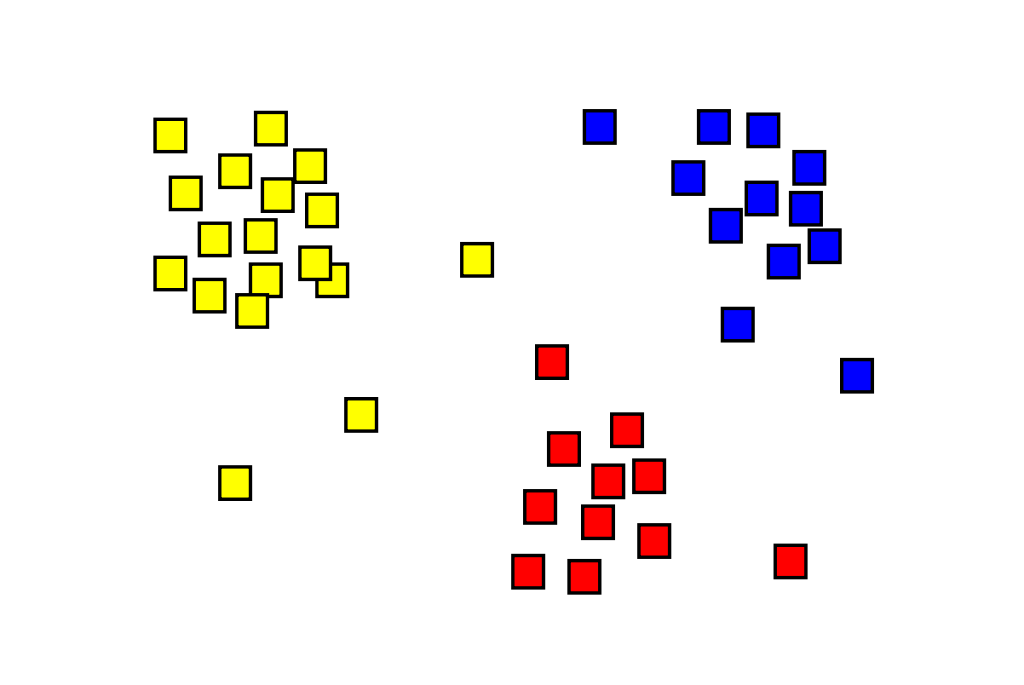
\includegraphics[width=0.3\textwidth]{clustering}
	\end{center}
	\begin{center}
		\vskip -0.5cm
		\caption{\small{El resultado de un análisis de grupo, mostrado como la coloración de cuadrados en tres grupos.}}
		{\small{Fuente: }}
	\end{center}
\end{figure}

Clustering es considerado una técnica de aprendizaje no supervisado puesto que busca encontrar relaciones entre variables descriptivas pero no la que guardan con respecto a una variable objetivo.


\subsubsection{Técnicas de clustering}

Existen dos grandes técnicas para el agrupamiento de casos:

\begin{itemize}
	\item Agrupamiento jerárquico: En este agrupamiento puede ser aglomerativo o divisivo.
	\item Agrupamiento no jerárquico: En este agrupamiento el número de grupos se determina de antemano y las observaciones se van asignando a los grupos en función de su cercanía. Existen los métodos de K-means y K-medoid.

\end{itemize}

\subsubsection{Algoritmos}

Existen diversas implementaciones de algoritmos concretos. Por ejemplo, el de las K-mediaso K-means. Es uno de los más antiguos pero su uso es muy extendido en la actualidad.
\vskip 1cm
El algoritmo de K-means es un algoritmo particional y fue propuesto en los ’50. Este algoritmo intenta encontrar una partición de nuestros ejemplos en \(K\) agrupaciones, de forma que cada ejemplo pertenezca a una de ellas, concretamente a aquella cuyo centro geométrico esté más cerca. El mejor valor de \(K\) para que la clasificación separe lo mejor posible los ejemplos no se conoce a priori, y depende completamente de los datos con los que trabajemos \citep{Jain}.
\vskip 1cm 
A pesar de que su primera aparición es desde hace más de 50 años sigue siendo de los algoritmos más utilizados para clustering por su facilidad de implementación, simpleza y buenos resultados empíricos.
\vskip 1cm 

\textbf{Los principales pasos del algoritmo son los siguientes:}

\begin{enumerate}
	\item Seleccionar una partición inicial (determinada por los centros de los clusters) con \(K\) clus-ters, repetir los pasos 2 y 3 hasta que los clusters se lleguen a estabilizar.
	\item Generar una nueva partición asignando cada dato al cluster cuyo centro está más cercano.	
	\item Calcular los nuevos centros de los clusters \(c(1)....c(K)\) (promediando los datos asignados a ese cluster en el paso anterior si la distancia es la euclídea).
\end{enumerate}

\textbf{El algoritmo K-medias requiere del usuario los siguientes parámetros:}

\begin{itemize}
	\item Número de clusters.
	\item Inicialización de los clusters (centros).
	\item Distancia (en general la distancia euclídea).
\end{itemize}

\begin{figure}[ht]
	\begin{center}
		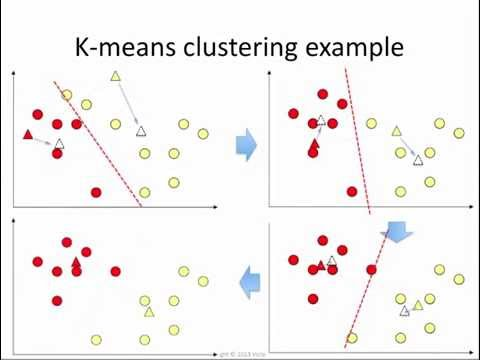
\includegraphics[width=0.8\textwidth]{proceso_kmeans}
	\end{center}
	\begin{center}
		\vskip -0.5cm
		\caption{\small{Proceso K-means.}}
		{\small{Fuente: }}
	\end{center}
\end{figure}


\subsubsection{Aplicaciones}

\begin{itemize}
	\item En marketing, para segmentar el mercado en pequeños grupos homogéneos donde realizar campañas publicitarias especificas.
	\item En biología, para dividir organismos en estructuras jerárquicas con el propósito de describir la diversidad biológica.
	\item En medicina, para diseñar tratamientos específicos para distintos grupos de riesgo.
	\item En psicología, para clasificar individuos en distintos tipos de personalidad, etc.
\end{itemize}

\subsection{Histograma}

\subsubsection{Definición}

Según \citep{histograma_unam} una histograma es una gráfica de la distribución de un conjunto de datos. Es un tipo especial de gráfica de barras y cada barra representa un subconjunto de los datos. Otra definición sostiene que un histograma es un gráfico de barras vertical que representa la distribución de frecuencias de un conjunto de datos \citep{histograma_aiteco}.

\vskip 1cm 
\subsubsection{Tipos}
Se agrupan los datos en clases, y se cuenta cuántas observaciones (frecuencia absoluta) hay en cada una de ellas. En algunas variables (variables cualitativas) las clases están definidas de modo natural, p.e sexo con dos clases: mujer, varón o grupo sanguíneo con cuatro: A, B, AB, O. En las variables cuantitativas, las clases hay que definirlas explícitamente (intervalos de clase) \citep{histograma_tipos}

\begin{itemize}
	\item \textbf{Simple:} Se representan los intervalos de clase en el eje de abscisas (eje horizontal) y las frecuencias, absolutas o relativas, en el de ordenadas (eje vertical).
	
	\begin{figure}[ht]
		\begin{center}
			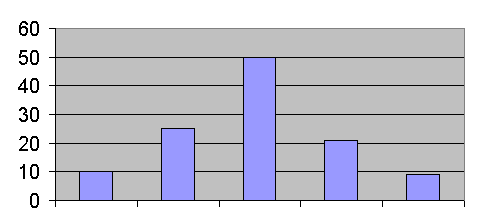
\includegraphics[width=0.8\textwidth]{histograma_simple}
		\end{center}
		\begin{center}
			\vskip -0.5cm
			\caption{\small{Histograma simple.}}
			{\small{Fuente: \citep{histograma_tipos}}}
		\end{center}
	\end{figure}
	
	\item \textbf{Por grupos:} Se representan simultáneamente los histogramas de una variable en dos situaciones distintas.
	
	\begin{figure}[ht]
		\begin{center}
			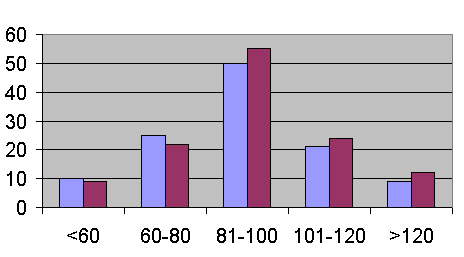
\includegraphics[width=0.8\textwidth]{histograma_grupos}
		\end{center}
		\begin{center}
			\vskip -0.5cm
			\caption{\small{Histograma por grupos.}}
			{\small{Fuente: \citep{histograma_tipos}}}
		\end{center}
	\end{figure}
	

	\item \textbf{Dirigido:} Se representan dos histogramas de la misma variable en dos situaciones distintas.
	
	\begin{figure}[ht]
		\begin{center}
			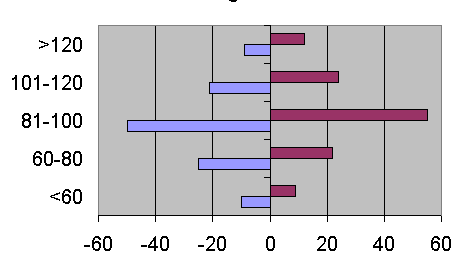
\includegraphics[width=0.8\textwidth]{histograma_dirigido}
		\end{center}
		\begin{center}
			\vskip -0.5cm
			\caption{\small{Histograma dirigidos.}}
			{\small{Fuente: \citep{histograma_tipos}}}
		\end{center}
	\end{figure}
	
	\item \textbf{Estratificado:} Se representan el conjunto dividido en subconjuntos, a cada subconjunto se le denomina estrato.
	
	\begin{figure}[ht]
		\begin{center}
			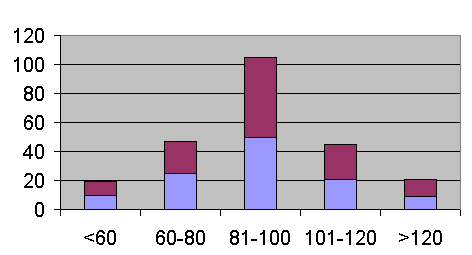
\includegraphics[width=0.8\textwidth]{histograma_estratificado}
		\end{center}
		\begin{center}
			\vskip -0.5cm
			\caption{\small{Histograma dirigidos.}}
			{\small{Fuente: \citep{histograma_tipos}}}
		\end{center}
	\end{figure}

\end{itemize}

\vskip 1cm 
\subsubsection{Utilidades}
\cite{histograma_tipos} nos indica las siguientes utilidades.
\begin{itemize}
	\item Proporciona, mediante el estudio de la distribución de los datos, un excelente punto de partida para formular hipótesis acerca de un funcionamiento insatisfactorio.
	\item El histograma es especialmente útil cuando se tiene un amplio número de datos que es preciso organizar, para analizar más detalladamente o tomar decisiones sobre la base de ellos.
	\item Es un medio eficaz para transmitir a otras personas información sobre un proceso de forma precisa e inteligible.
	\item Permite la comparación de los resultados de un proceso con las especificaciones previamente establecidas para el mismo. Ayuda a determinar si el proceso satisface los requisitos del cliente.
	\item Hace posible determinar si ha habido cambios en un proceso.
	
\end{itemize}


\subsection{Predicción}

\subsubsection{Definición}

El término predicción puede referirse tanto a la acción y al efecto de predecir como a las palabras que manifiestan aquello que se predice; en este sentido, predecir algo es anunciar por revelación, ciencia o conjetura algo que ha de sucede \citep{rae_prediccion}.
\vskip 0.2cm 
Predicción es una expresión que anticipa aquello que, supuestamente, va a suceder. Se puede predecir algo a partir de conocimientos científicos, revelaciones de algún tipo, hipótesis o indicios.

\subsubsection{Tipos}

\begin{description}
	\item [Científica:]
	\vskip 0.1cm 
	La predicción constituye una de las esencias claves de la ciencia, de una teoría científica o de un modelo científico. Así, el éxito se mide por el éxito o acierto que tengan sus predicciones \citep{mora_prediccion}.
	\vskip 0.1cm 
	La  predicción  en  el  contexto  científico  es  una  declaración  precisa  de  lo  que  ocurrirá  en determinadas  condiciones  especificadas.  Se  puede  expresar  a  través  del  silogismo:  "Si  A  es cierto, entonces B también será cierto".
	\vskip 0.1cm 
	El método científico concluye con la prueba de afirmaciones que son consecuencias lógicas del corpus de las teorías científicas. Generalmente esto se hace a través de experimentos que deben poder repetirse o mediante estudios observacionales rigurosos.
	\vskip 0.1cm 
	Una teoría científica cuyas aseveraciones no son corroboradas por las observaciones, por las pruebas o por experimentos probablemente será rechazada.
	 
	\item [Predicción no científica:]
	\vskip 0.1cm 
	Los para-psicólogos y los clarividentes, por su parte, apelan a pseudocientíficas para realizar predicciones. Estas personas dicen tener la posibilidad de conocer el futuro a partir de percepciones que reciben por sentidos que no son los cinco habituales (vista, olfato, gusto, oído y tacto). También hay sujetos que afirman recibir información por parte de entidades superiores(como dioses) para realizar sus predicciones \citep{julian_maria}
	\vskip 0.1cm 
	En estos casos, las predicciones no tienen ningún sustento lógico, por lo que creer en ellas suele ser una cuestión de fe o depender de la susceptibilidad de la persona.
	
\end{description}	
	

\subsection{Probabilidad}

\subsubsection{Definición}

La probabilidad es una medida de la certidumbre asociada a un suceso o evento futuro y suele expresarse como un número entre 0 y 1 (entre 0 \% y 100 \%). 
\vskip 0.1cm 
Una forma tradicional de estimar algunas probabilidades sería obtener la frecuencia de un acontecimiento determinado mediante la realización de experimentos aleatorios, de los que se conocen todos los resultados posibles, bajo condiciones suficientemente estables. Un suceso puede ser improbable (con probabilidad cercana a cero), probable (probabilidad intermedia) o seguro (con probabilidad uno) \citep{loeve}.

\subsubsection{Teoria de la probabilidad]}

Según \citep{alvarez_rojas} la probabilidad \(p\) de que suceda un evento \(S\) de un total de \(n\) casos posibles igualmente probables es igual a la razón entre el número de ocurrencias \(h\) de dicho evento (casos favorables) y el número total de casos posibles \(n\).

\begin{align*}
p = Prob(S) = \frac{h}{n}\\
\end{align*}

La probabilidad es un número (valor) que varia entre 0 y 1. Cuando el evento es imposible se dice que su probabilidad es 0, si el evento es cierto y siempre tiene que ocurrir su probabilidad es 1.
La probabilidad de no ocurrencia de un evento está dada por \(q\), donde:
\begin{align*}
p = Prob(noS) = 1 - \frac{h}{n}\\
\end{align*}


\subsubsection{Teoría de bayes}

El teorema de Bayes, en la teoría de la probabilidad, es una proposición planteada por el matemático inglés Thomas Bayes (1702-1761) \citep{bayes} y publicada póstumamente en 1763, que expresa la probabilidad condicional de un evento aleatorio A dado B en términos de la distribución de probabilidad condicional del evento B dado A y la distribución de probabilidad marginal de sólo A.
\vskip 0.1cm 
Las probabilidades Bayesianas se utilizan para encontrar la distribución de probabilidad condicional de un evento dados otros eventos , debido a su naturaleza se puede implementar al razonamiento bajo incertidumbre, los primeros estudios estaban basados en encontrar los errores sistemáticos en la estimación de probabilidades apoyados por la heurística, básicamente se da el análisis de la información que se utiliza para determinar la incertidumbre de la misma al realizar razonamientos probabilísticos, y encontrar el nivel de validez de los resultados obtenidos bajo esta perspectiva.

{\bf Formula de bayes:}\par

Con base en la definición de Probabilidad condicionada \citep{bayes_formula} se obtiene la Fórmula de Bayes, también conocida como la Regla de Bayes.
\vskip 0.5cm 
Sea ${ A 1 , A 2 , . . . , A i , . . . , A n }$ un conjunto de sucesos mutuamente excluyentes y exhaustivos, y tales que la probabilidad de cada uno de ellos es distinta de cero $(0)$. Sea B un suceso cualquiera del que se conocen las probabilidades condicionales $P ( B | A i )$. Entonces, la probabilidad $P ( A i | B )$ viene dada por la expresión: 

\[ P ( A i | B )  = \frac{P ( B | A i ) P ( A i )} {P ( B )} \]

{\bf Donde:}\par

\begin{description}
	\item[$P ( A i )$] son las probabilidades a priori.
	\item[$P ( B | A i )$] es la probabilidad de $B$ en la hipótesis $( A i )$
	\item[$P ( A i | B )$] son las probabilidades a posteriori. 
\end{description}

\subsection{Pregunta de opción múltiple}

La pregunta de opción múltiple o de selección múltiple o multiopción es una forma de
evaluación por la cual se solicita a los encuestados o examinados seleccionar una o varias de las opciones de una lista de respuestas.
\vskip 1cm 
Este tipo de pregunta es usado en evaluaciones educativas (en lo que popularmente se llaman exámenes tipo test), en elecciones (para escoger entre múltiples candidatos o partidos políticos diferentes), en los cuestionarios para estudios de mercado, encuestas, estadística y muchas otras áreas.

\begin{figure}[ht]
	\begin{center}
		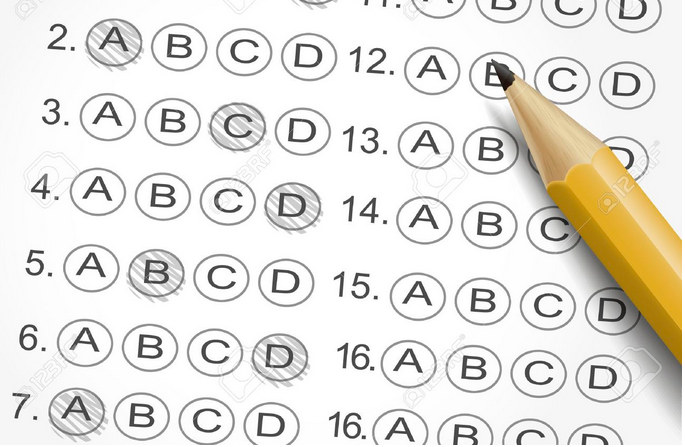
\includegraphics[width=0.8\textwidth]{pregunta_opcion_multiple}
	\end{center}
	\begin{center}
		\vskip -0.5cm
		\caption{\small{Hoja de respuestas de opción múltiple.}}
		{\small{Fuente: \citep{pregunta_opcion_multiple}}}
	\end{center}
\end{figure}
 
{\bf Formato:}\par

Un formato típico puede ser el de un enunciado seguido de una pregunta al respecto. El examinador ofrecerá normalmente de entre tres a cinco respuestas, típicamente a, b, c, d, e - de las cuales solamente una va a ser la respuesta correcta (la mejor respuesta) mientras las restantes respuestas serán los distractores \citep{salkind}
\vskip 1cm 


\subsection{Prototipo de software}

\subsubsection{Definición}

En Ingeniería de software un prototipo es una representación limitada del diseño de un producto que permite a las partes responsables de su creación experimentar su uso \citep{pressman_troya}, el prototipo debe ser construido en poco tiempo, usando los programas adecuados y no se debe utilizar muchos recursos.
\vskip 0.3cm
El diseño rápido se centra en una representación de aquellos aspectos del software que serán visibles para el cliente o el usuario final. Este diseño conduce a la construcción de un prototipo, el cual es evaluado por el cliente para una retroalimentación; gracias a ésta se refinan los requisitos del software que se desarrollará. La interacción ocurre cuando el prototipo se ajusta para satisfacer las necesidades del cliente. Esto permite que al mismo tiempo el desarrollador entienda mejor lo que se debe hacer y el cliente vea resultados a corto plazo \citep{pressman_troya}.


\subsubsection{Ventajas}

\begin{itemize}
	\item Este modelo es útil cuando el cliente conoce los objetivos generales para el software, pero no identifica los requisitos detallados de entrada, procesamiento o salida.
	\item También ofrece un mejor enfoque cuando el responsable del desarrollo del software está inseguro de la eficacia de un algoritmo, de la adaptabilidad de un sistema operativo o de la forma que debería tomar la interacción humano-máquina.
	\item Se puede reutilizar el código.
\end{itemize}

\subsubsection{Aplicación web}
En la ingeniería de software se denomina aplicación web a aquellas herramientas que los usuarios pueden utilizar accediendo a un servidor web a través de Internet o de una intranet mediante un navegador. En otras palabras, es una aplicación software que se codifica en un lenguaje soportado por los navegadores web en la que se confía la ejecución al navegador \citep{mora}.

\subsubsection{LAMP}

LAMP es el acrónimo usado para describir un sistema de infraestructura de internet que usa las siguientes herramientas:

\begin{itemize}
	\item Linux, el sistema operativo.
	\item Apache, el servidor web.
	\item MySQL/MariaDB, el gestor de bases de datos.
	\item Perl, PHP, o Python, los lenguajes de programación. 
\end{itemize}

La combinación de estas tecnologías es usada principalmente para definir la infraestructura de un servidor web, utilizando un paradigma de programación para el desarrollo \citep{apache}.
\vskip 0.3cm
A pesar de que el origen de estos programas de código abierto no han sido específicamente diseñado para trabajar entre sí, la combinación se popularizó debido a su bajo coste de adquisición y ubicuidad de sus componentes (ya que vienen pre-instalados en la mayoría de las distribuciones linux). Cuando son combinados, representan un conjunto de soluciones que soportan servidores de aplicaciones.

\subsubsection{Software}

\begin{itemize}
	\item \textbf{Linux:} Linux es un núcleo de sistema operativo libre tipo Unix.
	\item \textbf{Apache HTTP Server:} El servidor HTTP Apache es un servidor web libre y de código abierto, el más popular en cuanto a uso, sirviendo como plataforma de referencia para el diseño y evaluación de otros servidores web.
	\item \textbf{MySQL:} MySQL es un Sistema de Gestión de Bases de Datos (SGBD) relacional, que por 	lo tanto utiliza SQL, multihilo y multiusuario del que se estiman más de un millón de instalaciones.
	\item \textbf{PHP:} PHP (acrónimo recursivo de "PHP: Hypertext Preprocessor") es un lenguaje de programación diseñado para producir sitios web dinámicos. PHP es utilizado en aplicaciones del lado del servidor, aunque puede ser usado también desde una interfaz de línea de comandos o como aplicación de escritorio.
\end{itemize}

\begin{figure}[ht]
	\begin{center}
		
\includegraphics[width=0.8\textwidth]{LAMP_software}
	\end{center}
	\begin{center}
		\vskip -0.5cm
		\caption{\small{Software usado en LAMP.}}
		{\small{Fuente: }}
	\end{center}
\end{figure}



\chapter{Nombre de la propuesta o tema central de la tesis}

Basados en los conceptos discutidos en los capítulos 1 y 2. Se procederá a realizar el modelamiento de todo el proceso de predicción de la respuesta correcta, el desarrollo del algoritmo y de cada paso del proceso hasta llegar a resultado final.

\section{Desarrollo del algoritmo de aprendizaje no supervisado K-means} 

\subsection{Implementación}

\subsubsection{Diagrama de flujo}

El algoritmo tiene diferentes pasos en su proceso los cuales vemos en la Figura \ref{fig:steps_kmeans}

\begin{figure}[ht]
	\begin{center}
		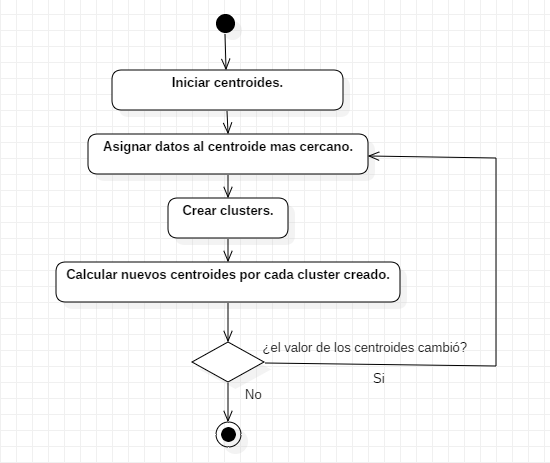
\includegraphics[width=0.8\textwidth]{steps_kmeans}
	\end{center}
	\begin{center}
		\vskip -0.5cm
		\caption{\small{Diagrama de actividades/flujo algoritmo Kmeans.}}
		{\small{Fuente: }}
	\end{center}
\end{figure}

\subsubsection{Pseudocodigo}
En la figura [] se muestra los pasos del algoritmo representado en Pseudocodigo.

\begin{algorithm}
\begin{algorithmic}[1]
		\REQUIRE Grupo de datos, Número de clusters.  % Entrada
		\label{lin:algorithm_kmeans}
		\ENSURE Centroides, Datos con sus respectivos clusters.                                                       % Salida
		
		\STATE Iniciar centroides.
					
		\STATE Asignar datos al centroide. \label{marker}
			
		\STATE Crear clusters.
			
		\STATE Calcular nuevos centroides por cada cluster creado.
			
		\IF {El valor de los centroides cambió}
			\STATE {\bf Goto} [ Paso 3]
		\ENDIF
			
		\RETURN  Centroides, Datos con sus respectivos clusters.
		
\end{algorithmic}
\end{algorithm}


\subsection{Proceso}

En esta sección se muestra el proceso que sigue K-means en las Figuras [] a través de todas las iteraciones que realiza hasta lograr que los grupos se puedan estabilizar en ese momento las iteraciones finalizan.

\begin{figure}[ht]
	\begin{center}
		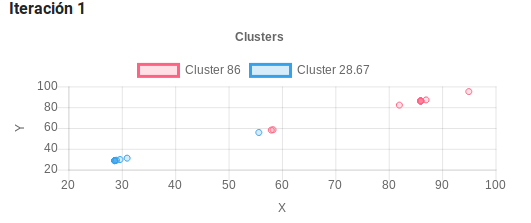
\includegraphics[width=0.8\textwidth]{step_kmeans_1}
	\end{center}
	\begin{center}
		\vskip -0.5cm
		\caption{\small{Grupos obtenidos en la iteración 1 .}}
		{\small{Fuente: Propia. }}
	\end{center}
\end{figure}

\begin{figure}[ht]
	\begin{center}
		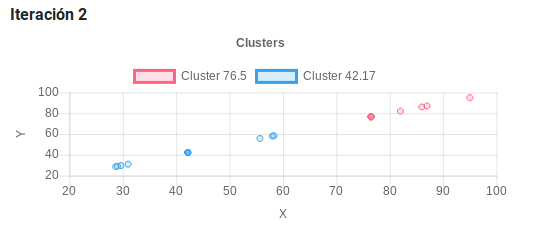
\includegraphics[width=0.8\textwidth]{step_kmeans_2}
	\end{center}
	\begin{center}
		\vskip -0.5cm
		\caption{\small{Grupos obtenidos en la iteración 2 .}}
		{\small{Fuente: Propia. }}
	\end{center}
\end{figure}

\begin{figure}[ht]
	\begin{center}
		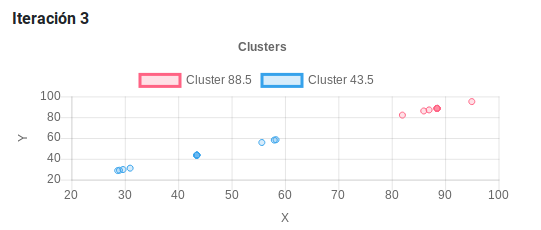
\includegraphics[width=0.8\textwidth]{step_kmeans_3}
	\end{center}
	\begin{center}
		\vskip -0.5cm
		\caption{\small{Grupos obtenidos en la iteración 3 (Final) .}}
		{\small{Fuente: Propia. }}
	\end{center}
\end{figure}


\section{Histograma}

\subsubsection{Diagrama de flujo}

El histograma tiene diferentes pasos en su proceso los cuales vemos en la Figura \ref{fig:steps_histogram}

\begin{figure}[ht]
	\begin{center}
		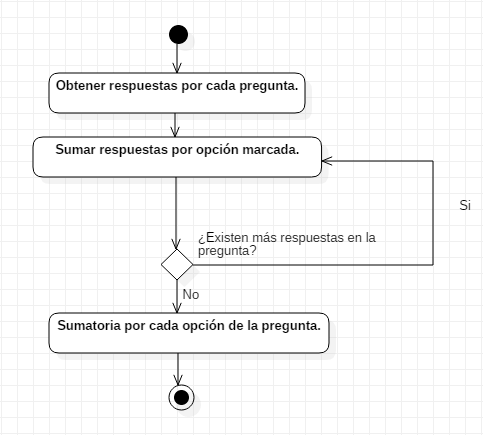
\includegraphics[width=0.8\textwidth]{steps_histogram}
	\end{center}
	\begin{center}
		\vskip -0.5cm
		\caption{\small{Diagrama de actividades/flujo Histograma. }}
		{\small{Fuente: Propia.}}
	\end{center}
\end{figure}

\subsubsection{Pseudocodigo}
En la figura [] se muestra los pasos representados en Pseudocodigo.

\begin{algorithm}
	\begin{algorithmic}[2]
		\REQUIRE Respuestas de una pregunta.  % Entrada
		\label{lin:algorithm_histogram}
		\ENSURE Sumatoria por cada opción de la pregunta .                                                       % Salida
		
		\STATE Obtener respuestas por pregunta.
		
		\STATE Sumar respuestas según la opción marcada. 
		
	
		\IF {Existen más respuestas en la pregunta}
		\STATE {\bf Goto} [ Paso 2]
		\ENDIF
		
		\RETURN  Sumatoria por cada opción de la pregunta.
		
	\end{algorithmic}
\end{algorithm}

\subsection{Proceso}

En esta sección se muestra el proceso donde se genera el histograma.























\section{Prototipo de aplicación web} 

\subsection{Modelamiento del proceso}

En esta sección vemos los pasos para poder realizar todo el proceso de la predicción de la respuesta correcta usando el prototipo desarrollado. En la figura \ref{fig:flow_chart_all_process} se muestra el diagrama de actividades de los procesos, la interaccion entre el usuario y el prototipo de aplicación web.

\begin{figure}[ht]
	\begin{center}
		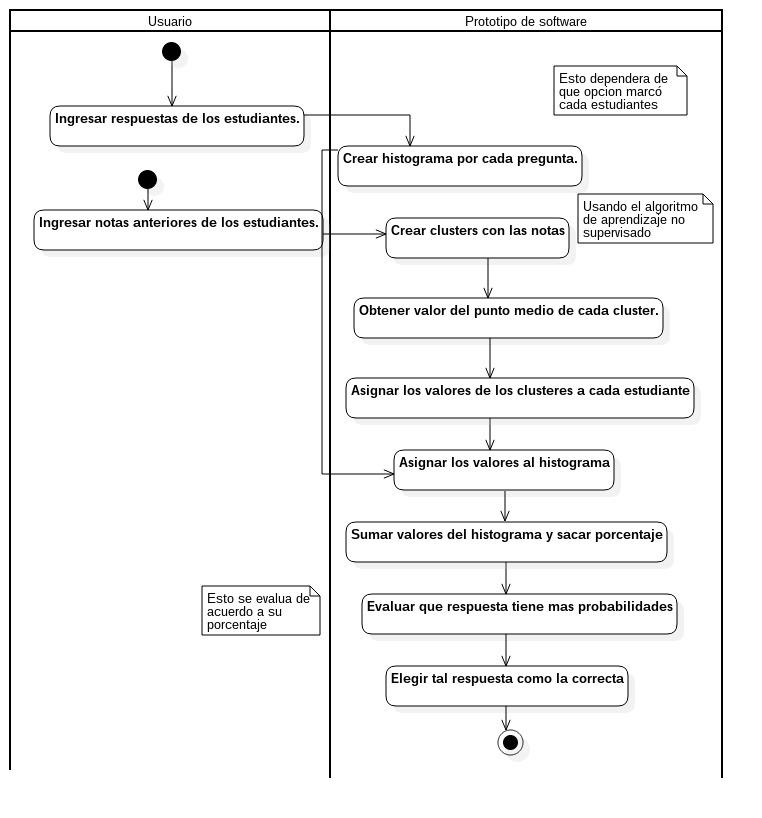
\includegraphics[width=0.8\textwidth]{flow_chart_all_process}
	\end{center}
	\begin{center}
		\vskip -0.5cm
		\caption{\small{Diagrama de actividades de todo el proceso.}}
		{\small{Fuente: }}
	\end{center}
\end{figure}


\subsection{Desarrollo}

El desarrollo del prototipo se realizo bajo un entorno Linux, usando Apache como servidor web, PHP como el lenguaje de servidor y HTML para la vistas. En la Figura 3.7 podemos ver la pantalla principal del prototipo donde muestra las diferentes opciones habilitadas. (MOSTRAR PANTALLA PRINCIPAL)

\subsection{Base de datos}
Algunos de los datos que se necesitan debían de ser permanentes, por lo cual se creo una pequeña base de datos para almacenarlos En la figura 3.8 vemos el diagrama relacional de la base de datos. (MOSTRAR DIAGRAMA DE LA BDD)


\section{Proceso para realizar la predicción} 

\subsection{Ejecutar K-means}

En la figura 3.9 se muestra los resultados de ejecutar K-means. Esta ejecución nos da como resultado los clusters ordenados. Mostrando los datos de los estudiantes, el promedio de sus notas, el cluster al que pertenecen y el valor de estos clusters.
(MOSTRAR RESULTADO DE LA EJECUCION KMEANS)

\subsection{Histograma por pregunta}

Por cada pregunta se obtiene cuantos estudiantes marcaron cada uno de las opciones, creando un histograma usando las respuestas por cada pregunta.

\subsubsection{Modelado}

El proceso del crear el histograma tiene diferentes pasos los cuales vemos en la Figura 3.10 \ref{fig:steps_histogram_process}

\begin{figure}[ht]
	\begin{center}
		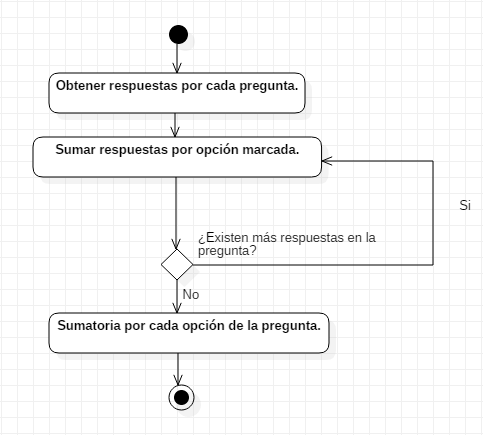
\includegraphics[width=0.8\textwidth]{steps_histogram}
	\end{center}
	\begin{center}
		\vskip -0.5cm
		\caption{\small{Pasos para el proceso del histograma.}}
		{\small{Fuente: Propia}}
	\end{center}
\end{figure}

\subsubsection{Modelado}

Se realizo la prueba de ejecución utilizando una pregunta de 4 opciones y con la respuesta de 7 estudiantes. En la figura 3.11 se muestra los resultados el histograma de una pregunta. En donde se muestra las opciones de la pregunta, el nombre los estudiantes que marcaron cada pregunta y el total de estudiantes por pregunta.
(MOSTRAR RESULTADO DEL HISTOGRAMA)

\subsection{Asignación valores de los clusters al histograma}

Después de haber obtenido el histograma de una pregunta, Se asigna el valor del cluster que pertenece a cada estudiante en el histograma, obteniendo la suma de ellos por cada opción. Luego se suman los resultados de todas las opciones para sacar un porcentaje por cada una y así la opción con mayor porcentaje sera elegida como la correcta. (EXPLICAR EL PROCESO)

\subsubsection{Modelado}

El proceso de asignar valores de los cluster al histograma tiene diferentes pasos los cuales vemos en la Figura \ref{fig:steps_asign_values_to_cluster}.

\begin{figure}[ht]
	\begin{center}
		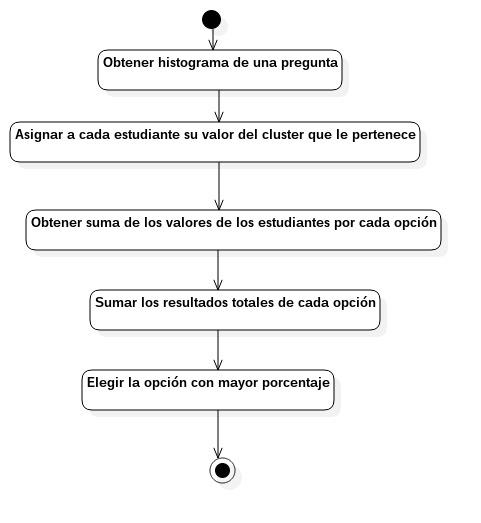
\includegraphics[width=0.8\textwidth]{steps_asign_values_to_cluster}
	\end{center}
	\begin{center}
		\vskip -0.5cm
		\caption{\small{Pasos para la asignación valores de los cluster al histograma.}}
		{\small{Fuente: Propia}}
	\end{center}
\end{figure}

\subsubsection{Resultado}

Se realizo la prueba de ejecución utilizando una pregunta de 4 opciones y con la respuesta de 7 estudiantes. En la figura 3.13 se muestra los resultados de la asignación valores de los 33cluster al histograma, mostrando también cual es la opción elegida como la correcta. En donde se muestra las opciones de la pregunta, el nombre los estudiantes que marcaron cada pregunta,
el total de estudiantes por pregunta, la suma de los valores de los clusters de cada estudiante por cada opción, el porcentaje de cada opción de la suma de los clusters y cual es la opción correcta según la que tiene mas porcentaje de la suma de los valores de los clusters. (MOSTRAR CAPTURA Y ARREGLAR TEXTO)


\section{Comparación de resultados} 

Las respuestas predecidas de cada preguntas se comparan con las respuestas correctas para poder obtener cuantas han sido predecidas correctamente.

\subsection{Resultado}

Se realizo la prueba de ejecución con 3 preguntas. La figura 3.14 muestra primero un resumen de cuantas predicciones de las respuestas de las preguntas fueron correctas y cuantas no Después muestra la lista de preguntas con su respuesta predecida, la respuesta que es la correcta y una opción que muestra si las 2 respuestas coinciden.
(MOSTRAR DONDE SE COMPRAN LAS PREGUNTAS)





















\section{Proceso de modelamiento} 

{\bf Ejemplo:}\par

La planificación y modelamiento del sistema de logística reversa de una área urbana es una fase importante y estratégica, para obtener en el futuro óptimos resultados en el proceso de gerenciamiento y operación del sistema reverso de RSU. El modelamiento permite determinar la localización de las estaciones de colecta y de unidades especiales necesarias, asi como el flujo que será movido a los largo de la red permitiendo dimensionar todo el sistema y sus componentes (Figura 3.1).
\vskip 0.3cm
\begin{figure}[ht]
\begin{center}
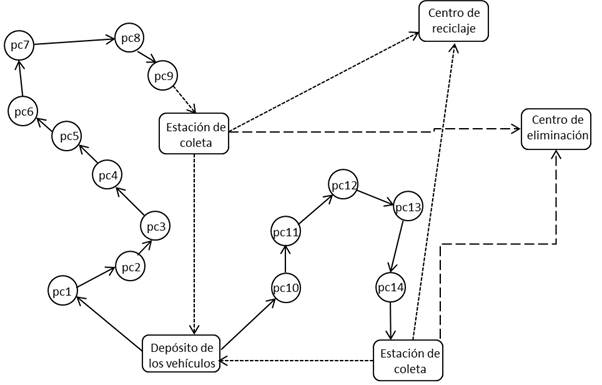
\includegraphics[width=.6\textwidth]{Figura3}
\end{center}
\begin{center}
\vskip -0.5cm
\caption{\small{Esquema del proceso de colecta y transporte de RSU.}}
{\small{Fuente: Elaboración propia}}
\end{center}
\end{figure}

\subsection{Proceso de ruteo}

\section{Implementación} 
























\chapter{Resultados y discusión de la tesis}


Al culminar con la investigación se llegaron a resultados interesantes del punto de vista tanto teórico como computacional. Estos resultados muestran que se contrasta la hipótesis planteada durante el proceso de elaboración del plan de investigación, es decir, que se logró demostrar la relación entre las variables de estudio formuladas en la investigación.

\section{Teóricos}

\section{Computacionales}




\chapter{Consideraciones finales}


\section{Conclusiones}

{\bf Ejemplo}\\
La investigación bibliográfica revela que realmente existe una preocupación de los gobiernos con el destino final de los residuos sólidos, con el objetivo de preservar la salud de la población y el medio ambiente urbano y rural. Por ejemplo, se observa la creación de la Ley 12305. Sin embargo existe una laguna entre las metas propuestas en la ley con las metas reales de los gobiernos locales. Eso se debe a la falta de una buena estructura organizacional, gerencial y operacional de los gobiernos locales capaz de atender las demandas locales y las necesidades de la población.
\vskip 0.3cm
La falta de cuadros especializados, tanto en los gobiernos centrales como locales, para realizar la planificación y modelamiento de una red logística reversa puede ser compensada con la contribución de los investigadores que actúan en ese campo del conocimiento. Es muy difícil la formación de un equipo que tenga todo el conocimiento en las áreas de ciencia de la computación, de geo procesamiento, de modelamiento matemático y de logística reversa, entre otras. Esa es una de las principales justificativas que los gobiernos, argumentan a la falta de planificación de una red logística reversa que funciones eficaz y eficientemente. 
\vskip 0.3cm
Por lo tanto, como quedó demostrado a lo largo de este trabajo, es posible realizar el modelamiento matemático para este tipo de problema con baja inversión, así como aplicarlo en varias regiones sin necesidad de grandes cambios en el modelamiento propuesto. El modelo propuesto calcula los flujos en la red logística reversa, permitiendo dimensionar la cantidad y capacidad de las unidades productivas y de los vehículos. 
\vskip 0.3cm
...


\section{Trabajos futuros}



\cleardoublepage
\addcontentsline{toc}{chapter}{Bibliografía}
\bibliographystyle{apalike}  % estilo de la bibliografía APA.
\bibliography{Bibliografia}   % Bibliografia.bib es el fichero donde está salvada la bibliografía.


